\documentclass[a4paper]{beamer}

\usepackage[english]{babel}
\usepackage[utf8]{inputenc}
\usepackage[T1]{fontenc}
\usepackage[english]{babel}
\usepackage{listings}

\usepackage{../thesis/sty/pgf-umlsd}

\usepackage{tikz}
\usetikzlibrary{positioning,shapes,arrows,chains,decorations.pathreplacing}

\lstset{
    numbers=left
}

% Template for talks using the Corporate Design of the Freie Universitaet
%   Berlin, created following the guidelines on www.fu-berlin.de/cd by
%   Tobias G. Pfeiffer, <tobias.pfeiffer@math.fu-berlin.de>
% This file can be redistributed and/or modified in any way you like.
%   If you feel you have done significant improvements to this template,
%   please consider providing your modified version to
%   https://www.mi.fu-berlin.de/w/Mi/BeamerTemplateCorporateDesign

\usepackage{amsmath,listings}

%%% FU logo
% small version for upper right corner of normal pages
\pgfdeclareimage[height=0.9cm]{university-logo}{resources/fu-logo}
\logo{\pgfuseimage{university-logo}}
% large version for upper right corner of title page
\pgfdeclareimage[height=1.085cm]{big-university-logo}{resources/fu-logo}
%%% end FU logo

\beamertemplatenavigationsymbolsempty

% NOTE: 1cm = 0.393 in = 28.346 pt;    1 pt = 1/72 in = 0.0352 cm
\setbeamersize{text margin right=3.5mm, text margin left=7.5mm}  % text margin

% colors to be used
\definecolor{text-grey}{rgb}{0.45, 0.45, 0.45} % grey text on white background
\definecolor{bg-grey}{rgb}{0.66, 0.65, 0.60} % grey background (for white text)
\definecolor{fu-blue}{RGB}{0, 51, 102} % blue text
\definecolor{fu-green}{RGB}{153, 204, 0} % green text
\definecolor{fu-red}{RGB}{204, 0, 0} % red text (used by \alert)

% switch off the sidebars
% TODO: loading \useoutertheme{sidebar} (which is maybe wanted) also inserts
%   a sidebar on title page (unwanted), also indents the page title (unwanted?),
%   and duplicates the navigation symbols (unwanted)
\setbeamersize{sidebar width left=0cm, sidebar width right=0mm}
\setbeamertemplate{sidebar right}{}
\setbeamertemplate{sidebar left}{}
%    XOR
% \useoutertheme{sidebar}

% frame title
% is truncated before logo and splits on two lines
% if neccessary (or manually using \\)
\setbeamertemplate{frametitle}{%
    \vskip-30pt \color{text-grey}\large%
    \begin{minipage}[b][23pt]{80.5mm}%
    \flushleft\insertframetitle%
    \end{minipage}%
}

%%% title page
% TODO: get rid of the navigation symbols on the title page.
%   actually, \frame[plain] *should* remove them...
\setbeamertemplate{title page}{
% upper right: FU logo
\vskip2pt\hfill\pgfuseimage{big-university-logo} \\
\vskip6pt\hskip3pt
% title image of the presentation
\begin{minipage}{11.6cm}
\hspace{-1mm}\inserttitlegraphic
\end{minipage}

% set the title and the author
\vskip14pt
\parbox[top][1.35cm][c]{11cm}{\color{text-grey}\inserttitle \\ \small \insertsubtitle}
\vskip11pt
\parbox[top][1.35cm][c]{11cm}{\small \insertauthor \\ \insertinstitute \\[3mm] \insertdate}
}
%%% end title page

%%% colors
\usecolortheme{lily}
\setbeamercolor*{normal text}{fg=black,bg=white}
\setbeamercolor*{alerted text}{fg=fu-red}
\setbeamercolor*{example text}{fg=fu-green}
\setbeamercolor*{structure}{fg=fu-blue}

\setbeamercolor*{block title}{fg=white,bg=black!50}
\setbeamercolor*{block title alerted}{fg=white,bg=black!50}
\setbeamercolor*{block title example}{fg=white,bg=black!50}

\setbeamercolor*{block body}{bg=black!10}
\setbeamercolor*{block body alerted}{bg=black!10}
\setbeamercolor*{block body example}{bg=black!10}

\setbeamercolor{bibliography entry author}{fg=fu-blue}
% TODO: this doesn't work at all:
\setbeamercolor{bibliography entry journal}{fg=text-grey}

\setbeamercolor{item}{fg=fu-blue}
\setbeamercolor{navigation symbols}{fg=text-grey,bg=bg-grey}
%%% end colors

%%% headline
\setbeamertemplate{headline}{
\vskip4pt\hfill\insertlogo\hspace{3.5mm} % logo on the right

\vskip6pt\color{fu-blue}\rule{\textwidth}{0.4pt} % horizontal line
}
%%% end headline

%%% footline
\newcommand{\footlinetext}{\insertshortinstitute, \insertshorttitle, \insertshortdate}
\setbeamertemplate{footline}{
\vskip5pt\color{fu-blue}\rule{\textwidth}{0.4pt}\\ % horizontal line
\vskip2pt
\makebox[123mm]{\hspace{7.5mm}
\color{fu-blue}\footlinetext
\hfill \raisebox{-1pt}{\usebeamertemplate***{navigation symbols}}
\hfill \insertframenumber}
\vskip4pt
}
%%% end footline

%%% settings for listings package
\lstset{extendedchars=true, showstringspaces=false, basicstyle=\footnotesize\sffamily, tabsize=2, breaklines=true, breakindent=10pt, frame=l, columns=fullflexible}
\lstset{language=Java} % this sets the syntax highlighting
\lstset{mathescape=true} % this switches on $...$ substitution in code
% enables UTF-8 in source code:
\lstset{literate={ä}{{\"a}}1 {ö}{{\"o}}1 {ü}{{\"u}}1 {Ä}{{\"A}}1 {Ö}{{\"O}}1 {Ü}{{\"U}}1 {ß}{\ss}1}
%%% end listings


\AtBeginSection[]
{
  \begin{frame}
    \tableofcontents[currentsection]
  \end{frame}
}

\author{Patrick Steinhardt}
\title{A Protocol for Connecting Distributed Resources}
\institute{Freie Universität Berlin}

\begin{document}

\begin{frame}[plain]
    \maketitle
\end{frame}

\begin{frame}
    \tableofcontents
\end{frame}

\section{Motivation}

\begin{frame}{Motivation}
    \begin{quote}
        The most profound technologies are those that disappear.
        They weave themselves into the fabric of everyday life until they are indistinguishable from it. \cite{weiser1991computer}
    \end{quote}
\end{frame}

\begin{frame}{Motivation}
    Provide a solution for connecting services with each other guaranteeing
    \begin{itemize}
        \item confidentiality of data sent
        \item authenticated identities
        \item controlability of services from a controlling device
    \end{itemize}
\end{frame}

\section{Architecture}

\begin{frame}{Architecture - Entities}
    Three kind of entities are taking part in the protocol:

    \begin{description}
        \item[Server]
            \begin{itemize}
                \item hosts different services
                \item responsible for answering service discovery
                \item owns a long term signature key pair
            \end{itemize}
        \item[Service]
            \begin{itemize}
                \item hosted on a server
                \item handles a service-specific protocol
            \end{itemize}
        \item[Client]
            \begin{itemize}
                \item user of one or multiple services
                \item owns a long term signature key pair
            \end{itemize}
    \end{description}
\end{frame}

\begin{frame}{Architecture - Sessions}
    \begin{itemize}
        \item using services requires a session
        \item sessions are created by clients
        \item sessions are deleted after being used
        \item sessions contain
            \begin{itemize}
                \item identifier
                \item session parameters
            \end{itemize}
        \item sessions are guarded by capabilities
    \end{itemize}
\end{frame}

\begin{frame}{Architecture - Capabilities}
    \begin{itemize}
        \item each sessions owns a root capability containing a secret
        \item from this secret, the server can generate referencing capabilities
        \item capabilities have access rights ``execute'' and ``terminate''
        \item capabilities are bound to public keys
        \item servers can cryptographically verify capabilities against the root capability
        \item based on identity-bound capabilities by Gong et al. \cite{gong1989secure}
    \end{itemize}
\end{frame}

\begin{frame}[fragile]{Architecture - Overview}
    \begin{figure}
        \centering

        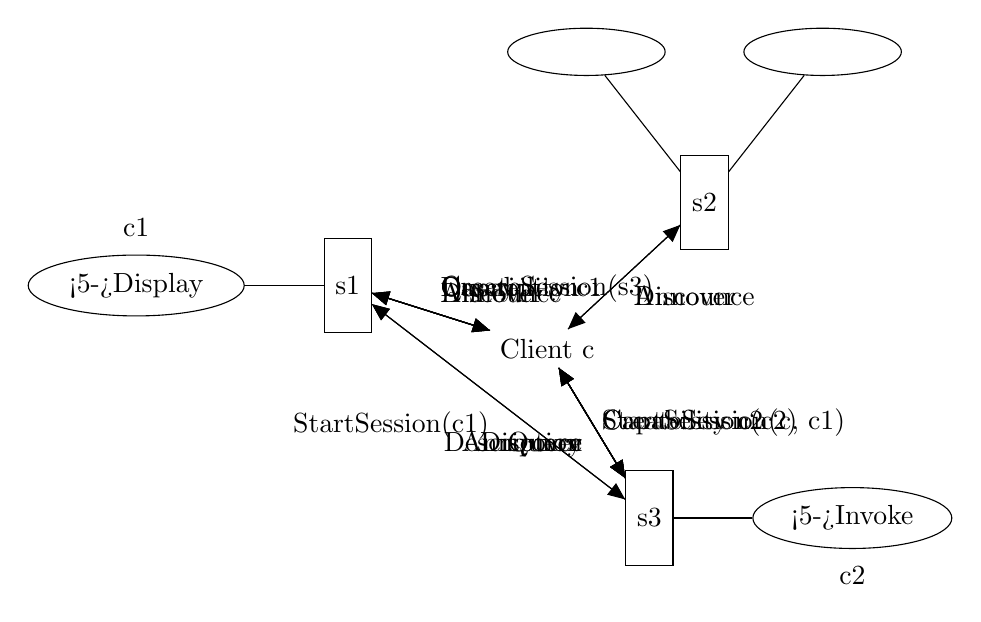
\begin{tikzpicture}[
                bidi/.style={draw, triangle 45-triangle 45},
                invoke/.style={draw, -triangle 45},
                server/.style={draw, rectangle, minimum height=1.2cm, minimum width=0.6cm},
                service/.style={draw, ellipse, minimum width=2cm, minimum height=0.6cm}
            ]

            \node (client) {Client c};

            \visible<3->{
                \node[server, left=1.5cm of client,  yshift=0.8cm] (s1) {s1};
                \node[server, above=1.0cm of client, xshift=2.0cm] (s2) {s2};
                \node[server, below=1.3cm of client, xshift=1.3cm] (s3) {s3};
            }

            % Discover
            \visible<2>{
                \path[invoke] (client) to node[above right] {Discover} (s1);
                \path[invoke] (client) to node[below right] {Discover} (s2);
                \path[invoke] (client) to node[below left] {Discover} (s3);
            }

            % Announce
            \visible<3>{
                \path[invoke] (s1) to node[above right] {Announce} (client);
                \path[invoke] (s2) to node[below right] {Announce} (client);
                \path[invoke] (s3) to node[below left] {Announce} (client);
            }

            % Services
            \visible<3->{
                \node[service, left=of s1] (display) {{\uncover<5->{Display}}};
                \path[draw] (display) -- (s1);

                \node[service, above=of s2, xshift=-1.5cm] (cpu2) {};
                \node[service, above=of s2, xshift=+1.5cm] (display2) {};
                \path[draw] (cpu2) -- (s2);
                \path[draw] (display2) -- (s2);

                \node[service, right=of s3] (invoke) {{\uncover<5->{Invoke}}};
                \path[draw] (invoke) -- (s3);
            }

            \visible<4>{
                \path[invoke] (client) to node[above right] {Query} (s1);
                \path[invoke] (client) to node[below left] {Query} (s3);
            }

            \visible<5>{
                \path[invoke] (s1) to node[above right] {Description} (client);
                \path[invoke] (s3) to node[below left] {Description} (client);
            }

            % CreateSession
            \visible<6>{
                \path[invoke] (client) to node[above right] {CreateSession(s3)} (s1);
            }
            \visible<7>{
                \path[invoke] (s1) to node[above right] {Capability c1} (client);
            }
            \visible<7-12>{
                \node[above=1mm of display] {c1};
            }

            % CreateSession
            \visible<8>{
                \path[invoke] (client) to node[right] {CreateSession(c, c1)} (s3);
            }
            \visible<9>{
                \path[invoke] (s3) to node[right] {Capability c2} (client);
            }
            \visible<9-10>{
                \node[below=1mm of invoke] {c2};
            }

            % StartSession
            \visible<10>{
                \path[invoke] (client) to node[right] {StartSession(c2)} (s3);
            }
            \visible<11->{
                \path[bidi] (client) to node[right] {} (s3);
            }

            % StartSession
            \visible<12>{
                \path[invoke] (s3) to node[below left] {StartSession(c1)} (s1);
            }
            \visible<13->{
                \path[bidi] (s3) to node[below left] {} (s1);
            }
        \end{tikzpicture}
    \end{figure}
\end{frame}

\section{Protocol}

\subsection{Low Level}

\begin{frame}{Protocol - Low Level - Wire Format}
    \begin{figure}
    \centering

    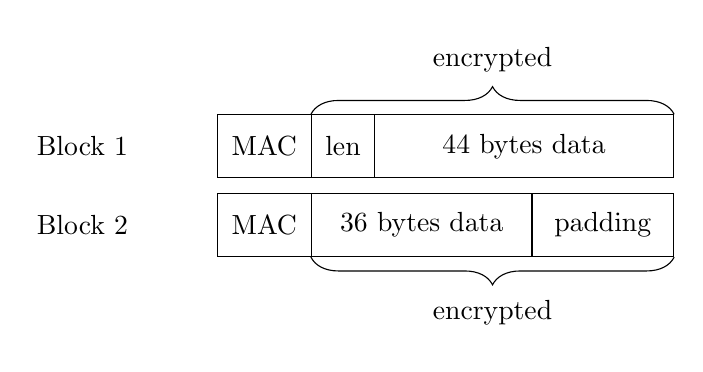
\begin{tikzpicture}[
            every node/.style={ minimum width=6mm, minimum height=8mm },
            start chain=1 going right,
            start chain=2 going right,
            node distance=-0.15mm
        ]

        \node[draw, on chain=1, minimum width=12mm] {MAC};
        \node[draw, on chain=1, minimum width=8mm ] {len};
        \node[draw, on chain=1, minimum width=38mm] {44 bytes data};
        \node[left=1cm of 1-1] {Block 1};

        \node[draw, on chain=2, minimum width=12mm, below=1cm of 1-1.west, anchor = west] {MAC};
        \node[draw, on chain=2, minimum width=28mm] {36 bytes data};
        \node[draw, on chain=2, minimum width=18mm] {padding};
        \node[left=1cm of 2-1] {Block 2};

        \draw [decorate,decoration={brace,amplitude=10pt}] (1-2.north west) -- (1-3.north east) node[midway,yshift=7mm] {encrypted};
        \draw [decorate,decoration={brace,amplitude=10pt,mirror}] (2-2.south west) -- (2-3.south east) node[midway,yshift=-7mm] {encrypted};
    \end{tikzpicture}
    \end{figure}
    \begin{itemize}
        \item fixed-length block format
        \item uses cryptographic primitives provided by NaCl crypto library \cite{nacl}
    \end{itemize}
\end{frame}

\begin{frame}{Protocol - Low Level - Message Format}
    \begin{itemize}
        \item based on Google Protocol Buffers \cite{varda2008protocol}
        \item message format specified via language-independent syntax
        \item compilers translate message formats to source code
    \end{itemize}
\end{frame}

\begin{frame}[fragile]{Protocol - Low Level - Key Agreement}
    \begin{itemize}
        \item each connection to a service requires setup of an encrypted connection
        \item initial connection authenticates identities and shared keys
        \item uses the SIG-DH authenticated key agreement protocol by Canetti et al. \cite{canetti2001analysis} to generate a shared symmetric key
        \item uses cryptographic primitives provided by NaCl crypto library \cite{nacl}
    \end{itemize}
\end{frame}

\subsection{Discovery}

\begin{frame}{Protocol - Discovery}
    \begin{columns}[t]
        \begin{column}{0.45\textwidth}
            \lstinputlisting[caption=Probe,firstline=16]{resources/proto/discovery.proto}
        \end{column}
        \begin{column}{0.45\textwidth}
            \lstinputlisting[caption=Answer,firstline=3,lastline=14]{resources/proto/discovery.proto}
        \end{column}
    \end{columns}
\end{frame}

\subsection{Query}

\begin{frame}{Protocol - Query}
    \begin{columns}[t]
        \begin{column}{0.45\textwidth}
        \end{column}
        \begin{column}{0.45\textwidth}
            \lstinputlisting[caption=Answer,firstline=14,lastline=21]{resources/proto/connect.proto}
        \end{column}
    \end{columns}
\end{frame}

\subsection{Session Handling}

\begin{frame}{Protocol - Session Establishment}
    \begin{columns}[t]
        \begin{column}{0.45\textwidth}
            \lstinputlisting[caption=Request,firstline=29,lastline=32]{resources/proto/connect.proto}
        \end{column}
        \begin{column}{0.45\textwidth}
            \lstinputlisting[caption=Answer,firstline=34,lastline=38]{resources/proto/connect.proto}
        \end{column}
    \end{columns}
\end{frame}

\begin{frame}{Protocol - Session Invocation}
    \begin{columns}[t]
        \begin{column}{0.45\textwidth}
            \lstinputlisting[caption=Request,firstline=39,lastline=41]{resources/proto/connect.proto}
        \end{column}
        \begin{column}{0.45\textwidth}
            \lstinputlisting[caption=Answer,firstline=47,lastline=49]{resources/proto/connect.proto}
        \end{column}
    \end{columns}
\end{frame}

\begin{frame}{Protocol - Session Termination}
    \begin{columns}[t]
        \begin{column}{0.45\textwidth}
            \lstinputlisting[caption=Request,firstline=43,lastline=45]{resources/proto/connect.proto}
        \end{column}
        \begin{column}{0.45\textwidth}
        \end{column}
    \end{columns}
\end{frame}

\section{Services}

\begin{frame}{Services}
    \begin{itemize}
        \item services are backed by plugins
        \item plugins can be registered dynamically
        \item five service plugins implemented
            \begin{description}
                \item[Capabilities] Request capabilities from an entity.
                \item[Invoke] Have a server execute another service.
                \item[Shell] Execute programs.
                \item[Synergy] Forward mouse- and keyboard-input.
                \item[Xpra] Forward graphical output to another computer.
            \end{description}
    \end{itemize}
\end{frame}

\subsection{Invoke}

\begin{frame}{Services - Invoke}

    \begin{figure}
        \centering

        \resizebox{0.8\textwidth}{!}
        {
            \begin{sequencediagram}
                \newthread{c}{Client c}
                \newinst[4]{s}{Service s}
                \newinst[4]{i}{Invoker i}

                \begin{call}{c}{CreateSession(i, Parameters p)}{s}{c1}
                    \begin{call}{s}{SaveSession(c, i, p)}{s}{Capability c1}
                    \end{call}
                \end{call}

                \postlevel

                \begin{call}{c}{CreateSession(c, c1)}{i}{c2}
                    \begin{call}{i}{SaveSession(c, c, c1)}{i}{Capability c2}
                    \end{call}
                \end{call}
                \postlevel

                \begin{messcall}{c}{StartSession(c2)}{i}
                    \begin{messcall}{i}{StartSession(c1)}{s}
                        \postlevel
                    \end{messcall}
                    \prelevel
                \end{messcall}
                \prelevel
            \end{sequencediagram}
        }
    \end{figure}
    \begin{description}
        \item[CreateSession(i, p)]\hfill\\
            Create session with invoker i and parameters p.
        \item[SaveSession(c, i, p)]\hfill\\
            Save session with creator c, invoker i and parameters p.
    \end{description}
\end{frame}

\subsection{Capabilities}

\begin{frame}{Services - Capabilities}
    \begin{figure}
        \centering

        \resizebox{0.8\textwidth}{!}
        {
            \begin{sequencediagram}
                \newthread{r}{Requester r}
                \newinst[2]{e}{Entity e}
                \newinst[3]{s}{Service s}
                \newinst[2]{c}{Capability Service}

                \mess{e}{Register}{c}
                \postlevel

                \begin{call}{r}{CapabilityRequest(e, s, params)}{c}{c1}
                    \postlevel
                    \begin{call}{c}{Ask(r, s, params)}{e}{c1}
                        \postlevel
                        \begin{call}{e}{CreateSession(r, params)}{s}{Capability c1}
                        \end{call}
                        \postlevel
                    \end{call}
                    \postlevel
                \end{call}

                \postlevel

                \begin{messcall}{r}{StartSession(c1)}{s}
                    \postlevel
                \end{messcall}

                \prelevel
            \end{sequencediagram}
        }
    \end{figure}
\end{frame}

\section{Implementation}

\begin{frame}{Implementation - Overview}
    \begin{columns}[t]
        \begin{column}{0.48\textwidth}
            \textbf{Server and command line client}

            \begin{itemize}
                \item builds on
                    \begin{itemize}
                        \item Windows
                        \item Linux
                        \item OS X
                    \end{itemize}
                \item continuous integration via Travis \cite{travis}, AppVeyor \cite{appveyor}
                \item static code analysis via Coverity \cite{coverity}
            \end{itemize}
        \end{column}
        \begin{column}{0.48\textwidth}
            \textbf{Android Controller}

            \begin{itemize}
                \item stepchild of the project
                \item continuous integration via Travis
                \item but: no tests
                \item works, but requires a lot of love
            \end{itemize}
        \end{column}
    \end{columns}
\end{frame}

\begin{frame}{Implementation - Source Code}
    \begin{columns}
        \begin{column}{0.48\textwidth}
            \begin{table}
                \centering
                \begin{tabular}{c|c|c}
                    Component & SLOC  & Test Cov\\
                    \hline
                    Core      & 2623 & $75\%$\\
                    Services  & 1132 & $7.3\%$\\
                    Exes      & 1301 & $0\%$\\
                    Tests     & 2361 & $100\%$\\
                    \hline
                    Total     & 8165 & $54.5\%$\\
                    &&\\
                    App       & 3409 & $0\%$
                \end{tabular}
                \caption{State at hand-in}
            \end{table}
        \end{column}
        \begin{column}{0.48\textwidth}
            \begin{table}
                \centering
                \begin{tabular}{c|c|c}
                    Component & SLOC  & Test Cov\\
                    \hline
                    Core      & 3121 & $80\%$\\
                    Services  &  974 & $38\%$\\
                    Exes      & 1277 & $0\%$\\
                    Tests     & 4364 & $100\%$\\
                    \hline
                    Total     & 9736 & $74.2\%$\\
                    &&\\
                    App       & 2386 & $0\%$
                \end{tabular}
                \caption{Current state}
            \end{table}
        \end{column}
    \end{columns}
\end{frame}

\begin{frame}{Implementation - What Changed}
    \begin{itemize}
        \item code quality
            \begin{itemize}
                \item libification of common source code
                \item improved tests for library functions
                \item tests for service plugins
                \item bug fixes
            \end{itemize}
        \item session parameters
            \begin{itemize}
                \item parameters are transmitted as protobufs instead of key-value-pairs
                \item parameters are verified on session establishment
                \item clients receive session parameters on connect
            \end{itemize}
        \item implementation of capability chains
        \item now hosted on \url{https://github.com/capone-project}
    \end{itemize}
\end{frame}

\begin{frame}{Implementation - What Remains}
    \begin{itemize}
        \item further cleanups
        \item more tests
        \item more service plugins
        \item better Android client
        \item better remote procedure call semantics
        \item server unification
    \end{itemize}
\end{frame}

\section{References}

\begin{frame}[allowframebreaks]{References}
    \bibliographystyle{plain}
    {\Tiny \bibliography{../thesis/resources/bibliography}}
\end{frame}

\begin{frame}[plain]
    \begin{center}
        Thank you for your attention.
    \end{center}
\end{frame}

\end{document}
